\documentclass[a4paper]{article}

\usepackage[utf8]{inputenc}
\usepackage[T1]{fontenc}
\usepackage{textcomp}
\usepackage[italian]{babel}
\usepackage{amsmath, amssymb}
\usepackage{siunitx}
\usepackage{caption}
\usepackage{graphicx}
\usepackage{subcaption}
\usepackage{amsmath}
\usepackage{booktabs} % Opzionale, per tabelle più belle se vuoi (\toprule, \midrule, \bottomrule)
\usepackage{ragged2e} % Per \Centering nelle minipage
\usepackage{float} % Per [htbp]

% ======================================================
% Impostazioni siunitx (opzionale, ma utile)
% ======================================================
\sisetup{
    output-decimal-marker = {,}, % Usa la virgola come separatore decimale
    uncertainty-mode = separate, % Mostra incertezza come ±
    separate-uncertainty = true, % Forza la separazione
    locale = IT % Impostazioni locali italiane (es. per la virgola)
}

% ======================================================
% Appendice con le tabelle dati
% ======================================================
\usepackage{appendix} % Usa il pacchetto appendix per una gestione migliore
\usepackage{titling}
\usepackage{appendix} % Pacchetto per l'appendice
\usepackage[colorlinks=true, linkcolor=blue, citecolor=blue, urlcolor=blue]{hyperref} % Per riferimenti cliccabili (opzionale ma utile)
\renewcommand{\appendixname}{Appendice} % Traduce "Appendix" in "Appendice"
\renewcommand{\appendixtocname}{Appendici} % Traduce "Appendices" nel ToC
\renewcommand{\appendixpagename}{Appendici} % Traduce "Appendices" nell'header/footer
\title{Circuiti 3 - Turno 2A - Gruppo 29}
\author{Emanuele Uriarte \and Michele Rota \and Sofia Zocchi}
\date{4 Aprile 2025}
\begin{document}

\maketitle

\section{Circuito RC} 
\subsection{Obiettivo}
Valutare la risposta in frequenza di un circuito RC alimentato da un generatore di segnale impostato su funzioni sinusoidali, ossia della forma 
$V_g = V_{0}  \cos(wt +\phi)$. Studiare sia l'andamento dell'ampiezza che della fase della funzione di trasferimento \footnote{$H(w)$: ci permette di descrivere la tensione in uscita (ai capi della resistenza o della capacità) come funzione della resistenza in entrata (ai capi del generatore)} per la tensione ai capi della resistenza e della capacità. 

\subsection{Metodo}
\begin{center}
	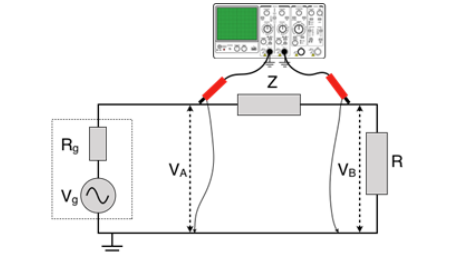
\includegraphics[width=0.5\textwidth]{grafici/circuito-rc.png}
	\captionof{figure}{Circuito RC}
	\label{fig:rc_circuito}
\end{center}
Per poter effettuare le misure abbiamo realizzato un circuito sulla breadbord come in figura \ref{fig:rc_circuito}. In questo caso $Z$ rappresenta la capacità $C$. Per poter campionare la forma d'onda di $V_c (t)$ e $V_R (t)$ abbiamo utilizzato un oscilloscopio a cui sono state collegate due sonde. Una sonda è stata posizionata in modo tale da misurare l'andamento di $V_g$, segnale sinusoidale, mentre l'altra è stata posizionata ai capi di $R$. Per misurare la caduta di potenziale ai capi della capacità $C$ abbiamo utilizzato la funzione $math$ dell'oscilloscopio la quale permette di eseguire operazioni matematiche con le onde in ingresso; nel nostro caso abbiamo impostato come operazione la sottrazione fra la tensione ai capi del generatore e la tensione ai capi della resistenza in modo da ottenere la tensione ai capi della capacità, infatti:
$V_g(t)=V_c(t)+V_R(t)$, dunque $V_c(t)=V_g(t)-V_R(t)$. Nell'ipotesi in cui $R$ e $C$ fossero state scambiate di posizione all'interno del circuito, i loro ruoli si sarebbero invertiti anche all'interno della definizione della differenza restituita dall'oscilloscopio.
Come resistenza abbiamo utilizzato una cassetta di resistenze che permette di scegliere un valore di $R$ arbitrario con un errore dell'1\%. Per misurare l'ampiezza e la fase delle onde abbiamo utilizzato la funzione $math$ dell'oscilloscopio: nel caso dell'ampiezza essa restituisce la distanza picco-picco, dunque il doppio dell'ampiezza di ciascuna onda mentre per quanto riguarda la fase misura lo sfasamento temporale tra il massimo di un onda in esame e il relativo massimo dell'onda di riferimento.

\subsection{Dati}
Per la realizzazione del circuito abbiamo impostato $R_{nota} = (10.0\pm 0.1) k\si{\ohm}$, in modo tale da poter considerare trascurabile sia la resistenza interna dell'oscilloscopio del generatore. La resistenza interna del generatore è infatti $\approx 1\si{\ohm}$, ed è collegata in serie ad $R_{nota}$, mentre $R_{osc}\approx 1M\si{\ohm}$ è collegata in parallelo a $R_{nota}$. Se considerassimo la resistenza equivalente dovuta alla presenza di $R_{osc}$ e $R_g$ essa si discosterebbe dal valore della resistenza impostata sulla cassetta in modo trascurabile rispetto all'errore stesso su $R_{nota}$. 
Per quanto riguarda invece la capacità inserita nel circuito ne abbiamo misurato il valore mediante un multimetro, ricavando $C_{nota} = (96 \pm 1) nF $.
Impostato $V_g(t)$ dal generatore abbiamo dapprima verificato che la forma d'onda erogata coincidesse con quanto restituito dall'oscilloscopio, dopodichè abbiamo misurato l'ampiezza della tensione ai capi del generatore mediante la funzionalità picco-picco. Fissato $V_g$, abbiamo poi raccolto circa 20 valori delle coppie $V_C - \nu$ e $V_R - \nu$, dove $V_C$ e $V_R$ indicano la distanza picco-picco per $V(t)$ ai capi della capacità e della resistenza, mentre $\nu$ indica la frequenza impostata sul generatore. Tale frequenza è stata scelta in un intorno della frequenza di taglio, stimata come $\nu_t = \frac{1}{2R_{nota}C_{nota}\pi}= 165.79 \si{\ohm}$. Utilizzando le medesime frequenze è stato misurato anche lo sfasamento $\Delta_{\phi_C}$ della funzione $V_C(t)$ e $\Delta_{\phi_R}$ di $V_R(t)$ rispetto a $V_g(t)$. Per quanto riguarda le incertezze abbiamo valutato i valori di frequenza come privi di errore, mentre abbiamo stimato l'errore sulle distanze picco-picco utilizzando la precisione dell'oscilloscopio, ossia metà dell'intervallo entro cui oscillavano i valori da esso restituiti.  Per quanto riguarda gli errori sulle fasi abbiamo deciso di considerare un errore del 5\% a causa dell'alta oscillazione dei valori dello strumento in fase di acquisizione dei dati. Ciò è riportato in tabella. 
%TODO inserire tabella con ampiezza vg, ampiezza vc, ampiezza vr, fase vc e fase vr in funzione della frequenza

\subsection{Analisi dati}
Dopo aver calcolato le pulsazioni $\omega=2\pi \nu$ abbiamo analizzato separatamente ampiezza e fase per valutare le funzioni di trasferimento $H_C(w)$ sulla capacità e $H_R(w)$ sulla resistenza. In entrambi i casi abbiamo considerato il rapporto della distanza picco-picco della tensione in uscita con quella della tensione in entrata, in modo tale da ottenere il rapporto tra le ampiezze. \footnote{La distanza picco-picco corrisponde al doppio dell'ampiezza, valutando il rapporto i fattori 2 però si semplificano}
Abbiamo quindi fittato i valori così ricavati con le funzioni che descrivono l'andamento atteso della funzione di trasferimento. Più precisamente dall'analisi circuitale e dall'applicazione del concetto di impedenza sono state ricavate le relazioni seguenti:
\begin{align}
|H_C|(\omega) = \frac{1}{\sqrt{1 + \omega^2R^2C^2}} \quad \text{,} \quad |H_R|(\omega) = \frac{\omega RC}{\sqrt{1 + \omega^2R^2C^2}}
\label{eq:ampiezza RC}\\
\arg(H_C(\omega)) = -\arctan(\omega RC) \quad \text{,} \quad \arg(H_R(\omega)) = \frac{\pi}{2}-\arctan(\omega RC)
\label{eq: fase RC}
\end{align}
Le relazioni riguadanti lo sfasamento delle funzioni di trasferimento possono considersi verificate a meno di multipli interi di $\pi$, ciò che è importante è infatti che $\arg(H_C(\omega))$ e $\arg(H_R(\omega))$ siano sfasati di $\frac{\pi}{2}$.
Quanto ricavato dai fit è osservabile nei grafici.
%TODO grafici ampiezze e fasi funzioni di trasferimento
Come si può osservare il circuito RC si comporta come un filtro passa basso, il modulo della funzione di trasferimento per la tensione ai capi della capacità è infatti massimo per basse frequenze (e quindi basse pulsazioni) e tende a 0 per valori molto alti di $\omega$.
Nella realizzazione del fit abbiamo fissato il parametro $R$, imponendo $R =R_{nota} = (10.0\pm 0.1) k\si{\ohm}$ e abbiamo ricavato il valore di $C_s$. 
I valori di capacità ricavati per ciascun fit sono riportati nella tabella.
%TODO tabella capacità ricavate per ciascun fit
Tali capacità sono state utilizzate per ottenere una stima empirica del valore di $C=$, calcolato mediante la media pesata, e del suo errore $\delta_{C_{media}}=$, corrispondente alla deviazione standard sulla media pesata.
Le capacità sono state confrontate mediante t-test; tra loro, con \( t = \frac {C_1 - C_2}{\sqrt{\delta_{C_1}^2+\delta_{C_2}^2}} \), e con $C_{att}$, con \( t = \frac {C_s - C_{att}}{\sqrt{\delta_{C_s}^2+\delta_{C_{att}}^2}} \). I risultati del test di compatibilità sono visibili in seguito, in tabella.
%TODO tabella t test per compatibilità capacità (tra quelle sperimentali e tra sperimentale e attesa)   
Nella realizzazione dei fit per le fasi delle funzioni di trasferimento è stato impostato un offset, corrispondente ad una traslazione sull'asse orizzontale. I valori di tale parametro ricavati mediante fit sono riportati in tabella. Il parametro $k_R$ (ricavato per il fit sulla fase di $H_R(\omega)$) risulta compatibile con una traslazione di $\frac{\pi}{2}$, come previsto dalla relazione \ref{eq: fase RC}. Al contrario il parametro $k_C$ (ricavato per il fit sulla fase di $H_C(\omega)$) risulta compatibile con un valore di $\pi$.
%TODO tabella offset fit fasi
Infine è stato valutato l'accordo tra i dati sperimentali e le funzioni di fit ricavate utilizzando il test del chi quadro, i cui esiti sono visibili nelle tabelle relative a ciascun fit.
%TODO tabelle chi quadro (o metterli dove ci pare)

\subsection{Conclusioni}
Basandoci sui risultati dei test del chi quadro possiamo affermare che le leggi ricavate per il modulo e le fasi della funzione di trasferimento offrono un buon accordo con i dati sperimentali sia per quanto riguarda $H_C(\omega)$ che per quanto riguarda $H_R(\omega)$. I risultati di $C$ ottenuti dalle funzioni di trasferimento interpolate risultano essere compatibili tra di loro, tuttavia essi non risultano essere compatibili con la capacità attesa misurata in laboratorio con il multimetro. 



\section{Circuito RL}
\subsection{Obiettivo}
Valutare la risposta in frequenza di un circuito RL alimentato da un generatore di segnale impostato su funzioni sinusoidali (della forma 
$Vg = V_{0} cos(wt + \phi)$). Studiare sia l'andamento dell'ampiezza che della fase della funzione di trasferimento per la tensione ai capi della resistenza e dell'induttanza.
\subsection{Metodo}
Per poter effettuare le misure abbiamo realizzato un circuito sulla breadbord come in figura \ref{fig:rc_circuito}. In questo caso $Z$ rappresenta l'induttanza $L$. Per poter campionare la forma d'onda di $V_L(t)$ e $V_R (t)$ abbiamo utilizzato un oscilloscopio a cui sono state collegate due sonde. Una sonda è stata posizionata in modo tale da misurare l'andamento di $V_g$, mentre l'altra è stata posizionata ai capi di $R$. Come effettuato per $C$, per misurare la caduta di potenziale ai capi dell'induttanza $L$ abbiamo utilizzato la funzione $math$ dell'oscilloscopio, più precisamente la differenza $V_L(t)=V_g(t)-V_R(t)$. Tale funzione ci ha anche permesso di campionare la distanza picco-picco (due volte l'ampiezza) delle varie onde e la loro fase rispetto a $V_g (t)$. Anche in questo caso la resistenza è stata scelta utilizzando la cassetta di resistenze, sulla quale è indicato un errore dell'1\% sul valore della resistenza scelta. 

\subsection{Dati}
Possiamo effettuare un ragionamento analogo al precente per quanto riguarda i valori di resistenza utilizzati, considerando trascurabili la resistenza interna dell'induttanza, dell'oscilloscopio e del generatore e deducendo quindi $R_{eq}\approx R_{nota} = (10.0\pm 0.1) k\si{\ohm}$. In quanto ignoto il valore dell'induttanza inserita nel circuito, non abbiamo potuto stimare la frequenza di taglio $\nu_t = \frac{R}{2\pi L}$. Abbiamo misurato la distanza picco-picco del segnale di tensione ai capi dell'induttanza e della resistenza per circa 15 valori di frequenza, al fine di campionare l'ampiezza delle funzioni di trasferimento. Per ricavarne invece la fase abbiamo osservato l'andamento dello sfasamento $\Delta_{\phi_L}$ (di $V_L (t)$) e $\Delta_{\phi_R}$ (di $V_R (t)$) rispetto a $V_g (t)$ in funzione della frequenza. I valori di $\nu$ impostati da generatore, e di conseguenza di $\omega= 2\pi \nu$, sono i medesimi. Come descritto per il circuito RC abbiamo considerato i valori di frequenza come privi di errore. Per determinare invece l'incertezza sull'ampiezza e lo sfasamento delle onde che descrivevano l'andamento della tensione ai capi dei vari elementi circuitali, abbiamo considerato la precisione con cui le misure venivano restituite dall'oscilloscopio. Unica eccezione consiste in quanto valutato per l'ampiezza della funzione di trasferimento sull'induttanza. In quest'ultimo caso per alte frequenze l'ampiezza di $V_L(t)$ (segnale in uscita) figurava maggiore di quella di $V_g(t)$ (segnale in entrata); evidenza sperimentale che ci ha portato ad ipotizzare che il circuito entrasse in risonanza, si comportasse cioè come circuito RLC, a causa della presenza delle capacità interne delle componenti del circuito, fino ad ora considerate trascurabili. Non potendo però confermare tale ipotesi ci siamo limitati a considerare un'incertezza maggiore sui valori della distanza picco-picco per la funzione $V_L(t)$. Quanto così ricavato è inserito in tabella.
%TODO inserire tabella con ampiezza vg, ampiezza vl, ampiezza vr, fase vl e fase vr

\subsection{Analisi dati}
Abbiamo quindi proceduto allo studio delle funzioni di trasferimento $H_L(w)$, la quale indica come la tensione fornita dal generatore si "trasferisce" sull'induttanza, e $H_R(w)$, la quale descrive invece come varia la tensione ai capi della resistenza. In entrambi i casi, per valutare il modulo della funzione di trasferimento, abbiamo considerato il rapporto della distanza picco-picco della tensione in uscita con quella della tensione in entrata. Per quanto riguarda invece le fasi il fit ha preso in considerazione direttamente i valori di $\Delta_{\phi}$ riportati nella tabella precedente.
L'andamento di ampiezze e fasi di $H(\omega)$ dipende dalla pulsazione $\omega$ secondo le relazioni: 
\begin{align}
	 & |H_L|(\omega) = \frac{\omega L}{\sqrt{R^2 + \omega^2L^2}}  \quad \text{,} \quad |H_R|(\omega) = \frac{R}{\sqrt{R^2 + \omega^2L^2}}\quad \label{eq:ampiezza RL}
\end{align}
\begin{align}
	 & <H_L(\omega) = \frac{\pi}{2} -arctg(\frac{\omega L}{R})  \quad \text{,} \quad <H_R(\omega) = -arctg(\frac{\omega L}{R}) \label{eq:fasi RL}
\end{align}
I risultati del fit effettuato sono riassunti nei grafici.
%TODO grafici fasi e ampiezze per circuito RL
Essi sono stati utilizzati per effettuare il test del chi quadro, atto a valutare la bontà del fit, i cui esiti sono raccolti in tabella.
%TODO tabella chi quadri
%CAPIRE PERCHè IL FIT PER L'AMPIEZZA DI VR FA SCHIFO MA VIENE SE SI TOLGONO ULTIMI 4 PUNTI (PROBLEMI CON FREQUENZE ALTE???)
Possiamo osservare come il circuito RL funzioni da filtro passa-alto, le armoniche ad alta frequenza passano infatti inalternate, con $|H_L|(\omega)$ che tende asintoticamente ad 1, mentre le armoniche a bassa frequenza vengono annullate: il modulo della funzione di trasferimento su $R_L$ diminuisce al diminuire della pulsazione (cioè della frequenza).


\subsection {Conclusione}
basandoci sui dati ottenuti mediante il test del chi quadro possiamo affermare che le leggi attese non offrono un buon accordo con i dati ottenuti sperimentalmente, nè per quanto riguarda i moduli delle funzioni di trasferimento $H_R(\omega)$ e $H_L(\omega)$ nè per quanto riguarda le fasi di tali funzioni. ciò è imputabile al fatto che l'oscilloscopio contiente una resistenza interna molto piccola, che va ad aggiungersi in parallelo al circuito RL. L'impedenza totale di questo circuito è $\frac{1}{Z_{eq}}=\frac{1}{R+Z_L}+Z_C$ con $C<<L$ e $C<<L$. Per $\omega$

\section{Circuito RLC}
\subsection{Obiettivo}
Valutare la risposta in frequenza di un circuito RLC alimentato da un generatore di segnale impostato su funzioni sinusoidali. Calcolare e studiare la funzione di trasferimento $H(\omega)$ per la tensione ai capi della resistenza, dell'induttanza e della capacità. Valutarne cioè sia l’andamento dell’ampiezza che della fase rispetto al segnale in entrata $V_g(t)=V_{0}  cos(wt +\phi)$.

\subsection{Metodo}
\begin{center}
	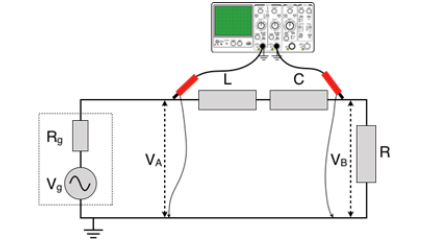
\includegraphics[width=0.5\textwidth]{grafici/circuito-rlc.png}
	\captionof{figure}{Circuito RLC}
	\label{fig:rlc_circuito} 
\end{center}
Innanzitutto abbiamo ricostruito il circuito rappresentato schematicamente in figura \ref{fig:rlc_circuito}; per farlo abbiamo collegato in serie induttore, capacitore e resistore, rappresentato dalla cassetta di resistenze. Abbiamo quindi utilizzato l'oscilloscopio per visualizzare l'andamento della tensione. Le sonde collegate all'oscilloscopio sono state collegate l'una in parallelo con il generatore, così da misurare $V_g$, e l'altra dapprima ai capi di $R$, poi ai capi di $C + R$, e infine ai capi di $L + R$. Mentre prima configurazione utilizzata ci ha permesso di misurare direttamente la caduta di potenziale $V_R$ ai capi della resistenza, le altre due sono state sfruttate in combinazione con la funzione $math$ dell'oscilloscopio, la quale ci ha permesso di misurare $V_L = V_g - (V_C + V_R)$ e $V_C = V_g - (V_L + V_R) $. Anche in questo caso per misurare l'ampiezza e la fase delle tensioni $V(t)$ al variare della frequenza $\nu$ impostata sul generatore, abbiamo utilizzato la funzione $math$ dell'oscilloscopio: essa restituisce la distanza picco-picco, dunque il doppio dell'ampiezza, e lo sfasamento temporale tra il massimo dell'onda in esame e il massimo più vicino di $V_g(t)$. Non siamo stati però in grado di campionare l'andamento della fase per $V_L$ e $V_C$, a causa della discontinuità e dell'incertezza dei valori restituiti dall'oscilloscopio. 
Tutte le misurazioni sono state effettuate impostando sulla cassetta di resistenze un valore di $R$ che determinava l'instaurarsi di un regime sovrasmorzato; ciò è stato osservato variando la forma del segnale da sinusoidale a onda quadra e valutando quanto restituito dall'oscilloscopio sulla base dell'esperienza di laboratorio precedente.

\subsection{Dati}
In quanto sono state utilizzate tre configurazioni di misura differenti abbiamo ottenuto per la tensione ai capi della resistenza, dell'induttanza e della capacità valori dipendenti da frequenze tra loro differenti. Indicativamente si sono scelte frequenze comprese tra qualche decina e qualche centinaia di migliaia di Hertz. Inoltre è stato fondamentale osservare che al variare della frequenza impostata dal generatore l'oscilloscopio registrava leggere variazioni della distanza picco-picco della tensione in entrata $V_g$, seppur l'ampiezza di quest'ultima non venisse variata. Abbiamo quindi appuntato queste variazioni così da tenerne conto nel calcolare i rapporti $V_L/V_g$, $V_C/V_g$ e $V_R/V_g$, ossia i moduli delle funzioni di trasferimento. Nella tabella sono riportati i valori delle distanza picco-picco per la tensione $V_g$, $V_L$, $V_C$ e $V_R$ e dello sfasamento $\Delta_{\phi_R}$ (di $V_R (t)$) rispetto a $V_g (t)$ e i relativi errori, in funzione della frequenza $\nu$. Per quanto riguarda la stima delle incertezze abbiamo osservato gli intervalli entro cui l'oscilloscopio restituiva i valori delle distanze picco-picco e degli sfasamenti.
%TODO 3 tabelle (PERCHè LE FREQUENZE E LE VG SONO DIVERSE NEI 3 CASI):
%1 frequenza vg, vr, sfasamento di vr
%2 frequenza vg, vl
%3 frequenza vg, vc

\subsection{Analisi dati}
A partire dai dati sperimentali abbiamo ricavato la pulsazione $\omega = 2\pi \nu$ e le ampiezze delle funzioni di trasferimento dalle realazioni $|H_R|(w)= \frac{V_R}{V_g}$, $|H_L|(w)= \frac{V_L}{V_g}$ e $|H_R|(w)= \frac{V_R}{V_g}$. 
Per tali grandezze è stato eseguito un fit utilizzando la forma funzionale delle funzioni di trasferimento attese, sia per l'ampiezza che per lo sfasamento. In seguito riportiamo le relazioni ricavate a partire dall'analisi circuitale del circuito RLC e dalla rappresentazione delle sue caratteristiche mediante coefficienti complessi (impedenze).
\begin{align}
	 &|H_L|(\omega) = \frac{\omega L}{\sqrt{R^2 + (\omega L-\frac{1}{\omega C})^2}} \quad \text{,} \quad |H_C|(\omega) = \frac{1}{\omega C\sqrt{R^2 + (\omega L-\frac{1}{\omega C})^2}} \quad \label{eq:ampiezze VL, Vc RLC}
\end{align}
\begin{align}
	 &  |H_R|(\omega) = \frac{R}{\sqrt{R^2 + (\omega L-\frac{1}{\omega C})^2}}  \quad \text{,} \quad <H_R(\omega) = -arctg(\frac{\omega L -\frac{1}{WC}}{R}) \label{eq:Vr_RLC}
\end{align}
Per ogni fit abbiamo considerato come noto il valore della resistenza equivalente del circuito $R_{eq}\approx R_{nota} = (10.0\pm 0.1) k\si{\ohm}$, approssimabile appunto alla resistenza impostata manualmente in quanto rispetto ad essa la resistenza interna dell'oscilloscopio (collegata in parallelo), del generatore e dell'induttanza (collegate in serie) risultavano trascurabili. L'esito dei fit realizzati è visualizzabile nel grafico.
%TODO grafici fit RLC nell'ordine: ampiezza per vl, ampiezza per vc, ampiezza per vr, fase per vr
Come è possibile osservare dalla forma del modulo della funzione di trasferimento per la tensione ai capi della resistenza $|H_R(j\omega)|$, essa ha la forma di una risonanza. La funzione ha valore massimo, pari ad 1, in corrispondenza della frequenza di risonanza, cioè per $\omega = \frac{1}{\sqrt{LC}}$.
Inoltre possiamo ricavare nformazioni sulla risposta in frequenza del circuito anche dalla larghezza $\Delta \omega$ della curva $|H_R(j\omega)|$. Tale larghezza corrisponde alla differenza tra le 2 frequenze di taglio ed è pari a $\Delta \omega = \frac{R}{2\pi L}$. Al suo aumentare, cioè all'aumentare di $R$ o al diminuire di $L$, la risposta sulla resistenza risulta meno “selettiva “.
Infatti il modulo di $H_R(j\omega)$ decresce più lentamente; si ha quindi anche il passaggio di armoniche a frequenze più distanti dalla frequenza di risonanza, esse cioè non vengono annullate.

L'analisi delle misure effettuate ci ha poi permesso di ricavare empiricamente i valori di capacità e induttanza, osservabili in tabella.
%TODO tabelle capacità e induttanze ricavate sperimentalmente per ciascun fit
Tali risultati sono stati confrontati con i valori di $C_{media}$, proveniente dallo studio del circuito RC, e $L_{media}$, calcolato invece in seguito all'esperienza col circuito RL. Il confronto è stato effettuato mediante t-test, il quale ci ha permesso di valutare la compatibilità tra i risultati ottenuti mediante modalità differenti. Si sono utilizzate la relazioni  \( t = \frac {C_{media} - C_s}{\sqrt{\delta_{C_{media}}^2+\delta_{C_s}^2}} \) e \( t = \frac {L_{media} - L_s}{\sqrt{\delta_{L_{media}}^2+\delta_{L_s}^2}} \), dove ($C_s \pm  \delta_{C_s}$) e ($L_s \pm  \delta_{L_s}$) sono stati ricavati dai fit per il circuito RLC, mentre $\delta_{C_{media}}$ e $\delta_{L_{media}}$ indicano la deviazione standard sulla media pesata delle misure ricavate dai fit di RC e RL. I risultati ottenuti sono raccolti in tabella.
%TODO tabelle t test tra le c ricavate sperimentalmente da RLC e la c media ricavata da RC
%TODO tabelle t test tra le L ricavate sperimentalmente da RLC e la L media ricavata da RL
Per valutare poi la bontà dei fit effettuati abbiamo realizzato il test del chi quadro, con esiti visibili in tabella.
% TODO tabella chi quadri

\subsection{Conclusione}




\end{document}